% !TEX root = main.tex
\pagenumbering{roman}

\begin{titlepage}
\begin{center}
\ \\

\vspace{15mm}

\large
Charles University in Prague\\
Faculty of~Mathematics and Physics\\

\vspace{5mm}

{\Large\bf MASTER THESIS}

\vspace{15mm}


\includegraphics[scale=0.4]{logo.eps} %%% source http://www.mff.cuni.cz/fakulta/symboly/logo.eps

\vspace{20mm}
%\normalsize
{\Large Ondřej Plátek}\\ 

\vspace{5mm}
{\Large\bf Automatic speech recognition using Kaldi}

\vspace{20mm}
\large
\noindent
Institute of~Formal and Applied Linguistics\\
\noindent
Supervisor: Ing. Mgr. Filip Jurčíček, Ph.D.\\
\noindent
Study branch: Theoretical Computer Science\\
\end{center}
\vspace{20mm}
\begin{center}
Prague 2013
\end{center}

\end{titlepage} % zde koncí úvodní strana

%%%%%%%% 2-3 page with master thesis task
% FIXME -remove this from electronic version%%%%% 
\todon{Insert the~task $../images/zadani[1-2].png$ for the~printed version}
\newpage
%%%%%%%% end 2-3 page with master thesis task

%%% 4.(2.) title page
\normalsize % nastavení normální velikosti fontu
\vspace{10mm} 

\noindent I would like to thank my~supervisor, Ing. Mgr. Filip Jurčíček, Ph.D., for his advice, guidence and keeping me
motivated. Many thanks to my~friends from Rotunda Lab, Dialog System group and Ada for being supportive.
I would like to thank namely, Matej Korvas for HTK scripts results and advices, 
Lukas Zilka, David Marek and Ondrej Dusek for hacks in Vim, Bash and Perl, 
Marek Vasut for advices with shared library linking and Tomas Martinec for C++ advices.
I am also very grateful to the~Kaldi team, which was very responsive and helpful.
Expecially, Daniel Povey and  Vassil Panayotov. 
Last but not least, I would like to thank my~parents for all the~help and support.


\vspace{\fill} % nastavuje dynamické umístění následujícího textu do spodní části stránky
\noindent
I declare that I wrote my master thesis independently and exclusively with~the~use of~the~cited sources. I agree with~lending and publishing this thesis.

%\medskip\noindent
%I acknowledge that my thesis is a~subject to the~stipulations of~rights and obligations of~the~Act No. 121/2000 Coll., Copyright Act as valid, especially the~fact that Charles University in~Prague has a right to conclude a~licence agreement on~the~use of~the~school work as per sect. 60, paragraph 1 of~the~Copyright Act.

\medskip\noindent
I declare that I carried out this master thesis independently, and only with the~cited sources, literature and other professional sources.

I understand that my work relates to the~rights and obligations under the~Act No. 121/2000 Coll., the~Copyright Act, as amended, in particular the~fact that the~Charles University in Prague has the~right to conclude a license agreement on the~use of~this work as a school work pursuant to Section 60 paragraph 1 of~the~Copyright Act.

\noindent Prague, August 1, 2013 \hspace{\fill}Ondřej Plátek 

%%%   Výtisk pak na tomto míst+ nezapomente PODEPSAT!
%%%                                         *********

%\begin{figure}[htp] \centering{
%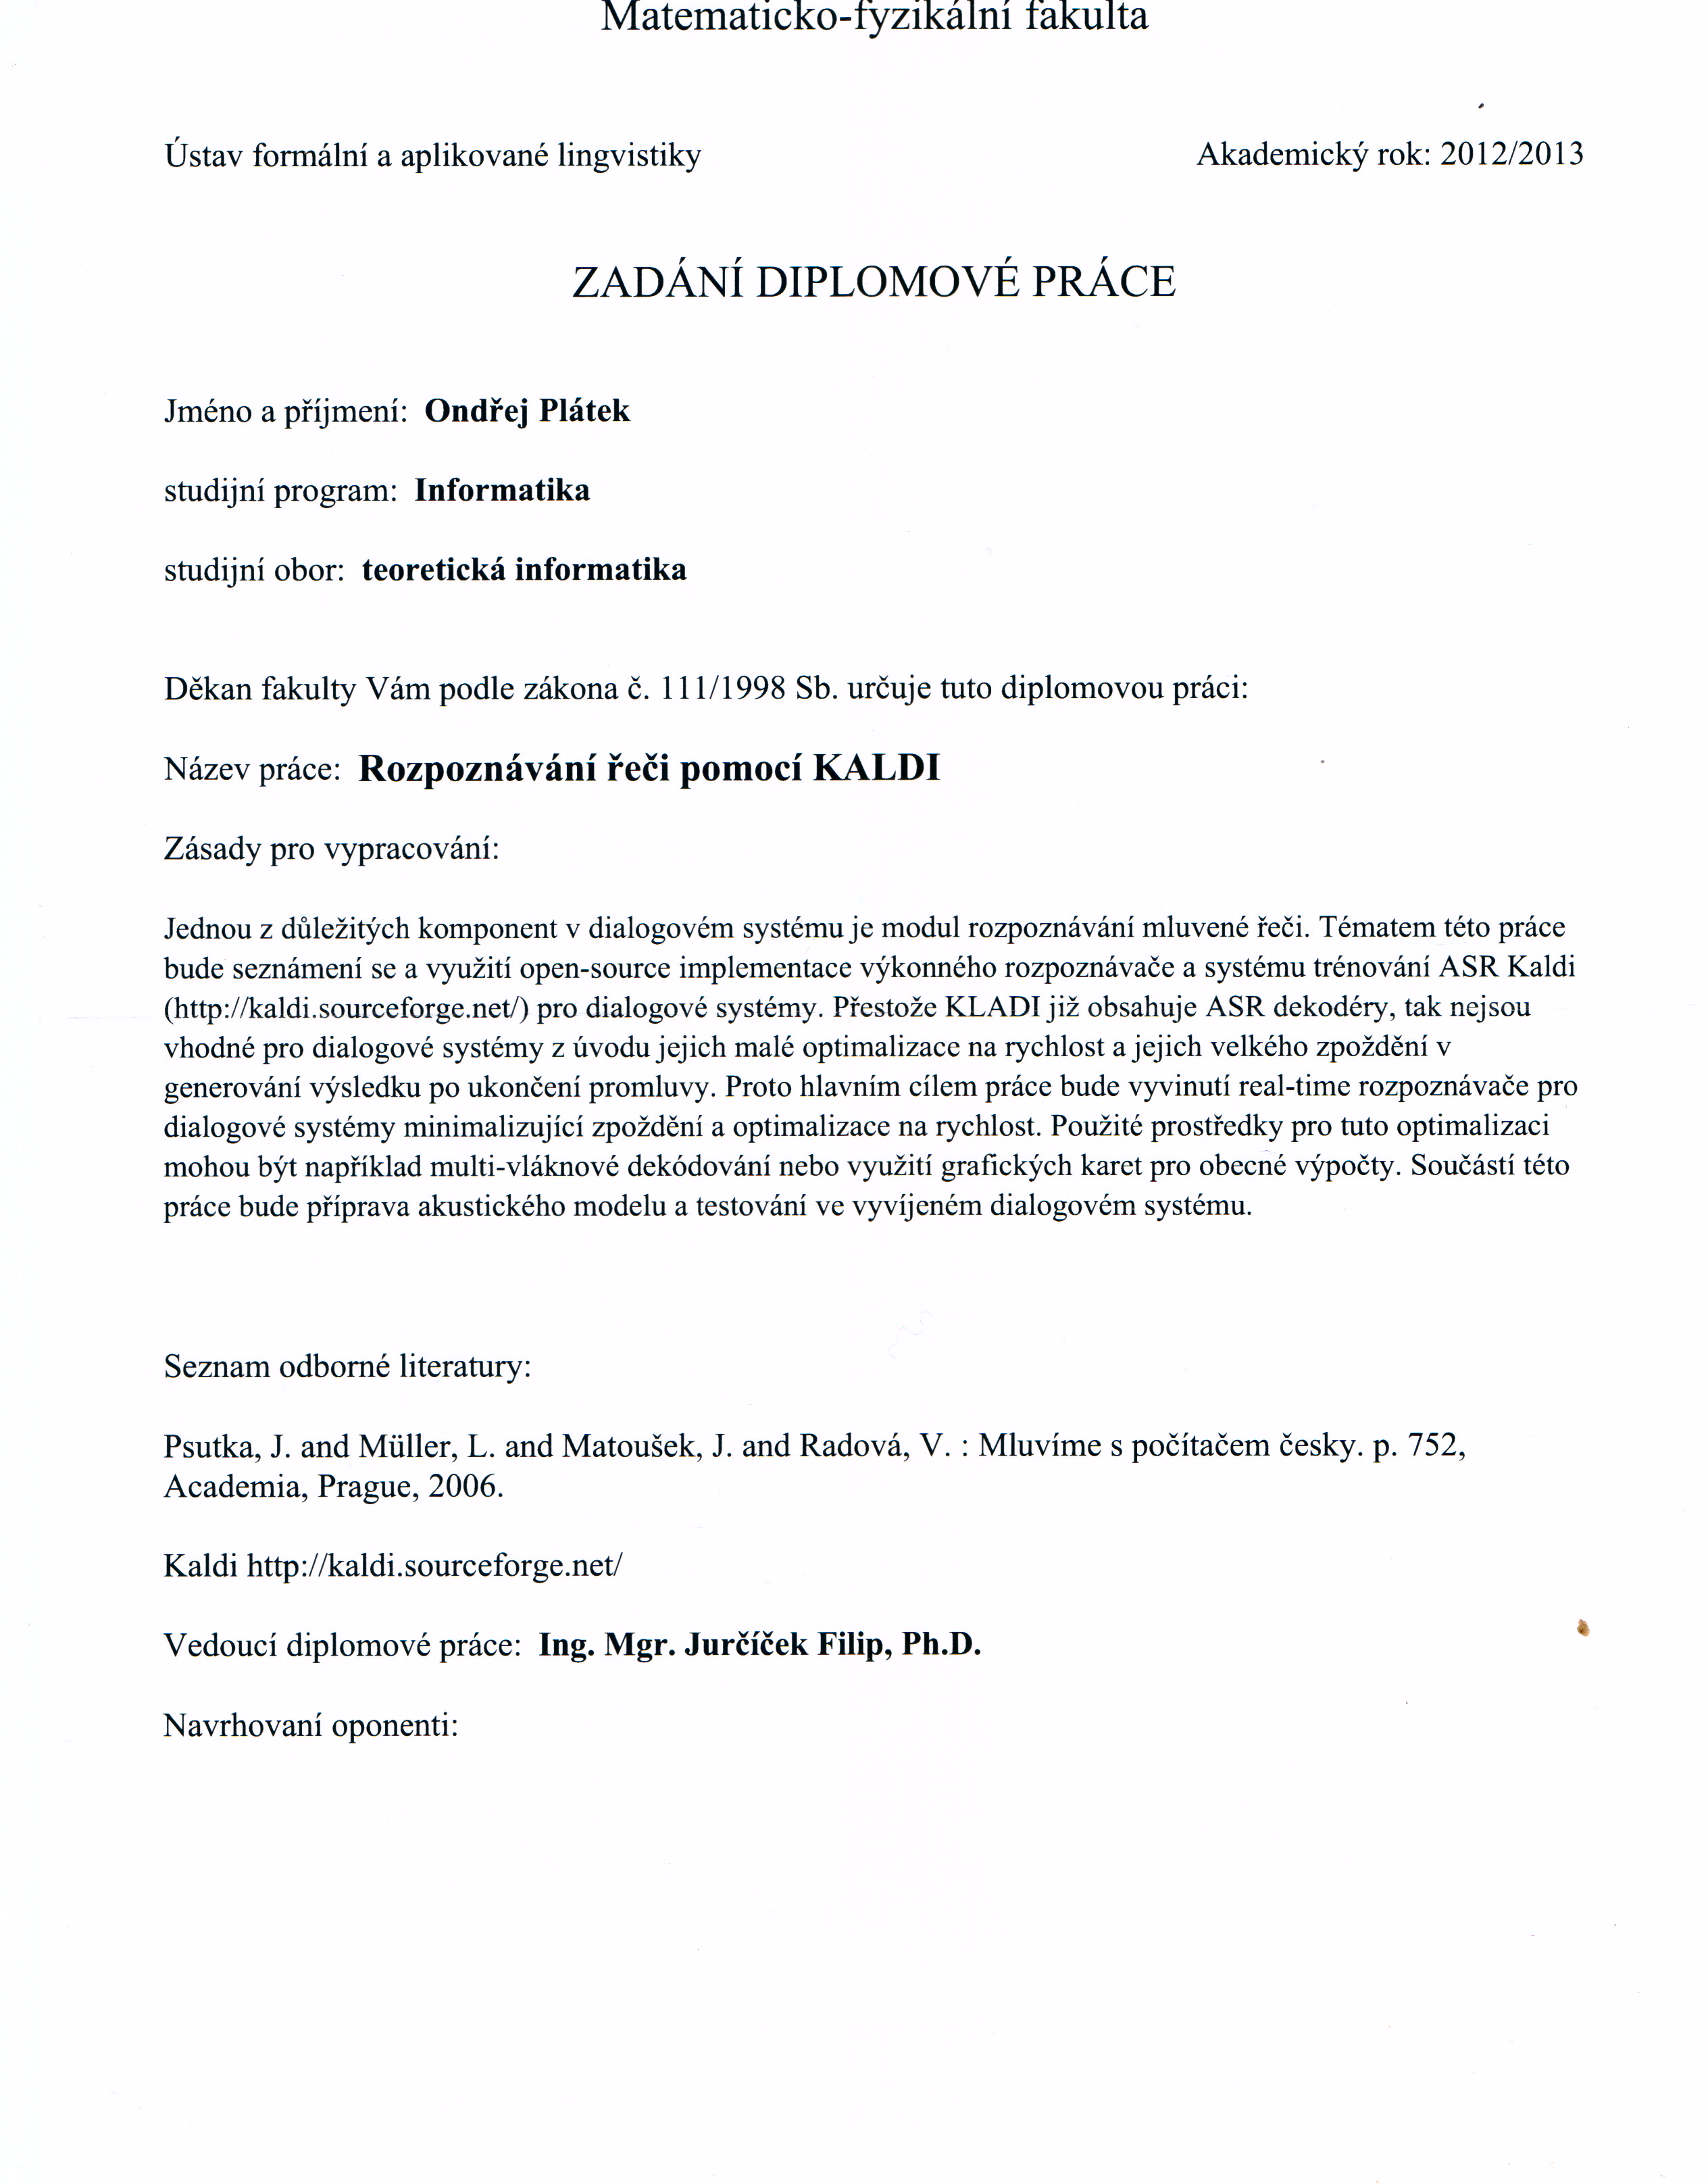
\includegraphics[scale=0.82]{zadani1}}
%\end{figure}  
%
%\newpage
%\begin{figure}[htp] \centering{
%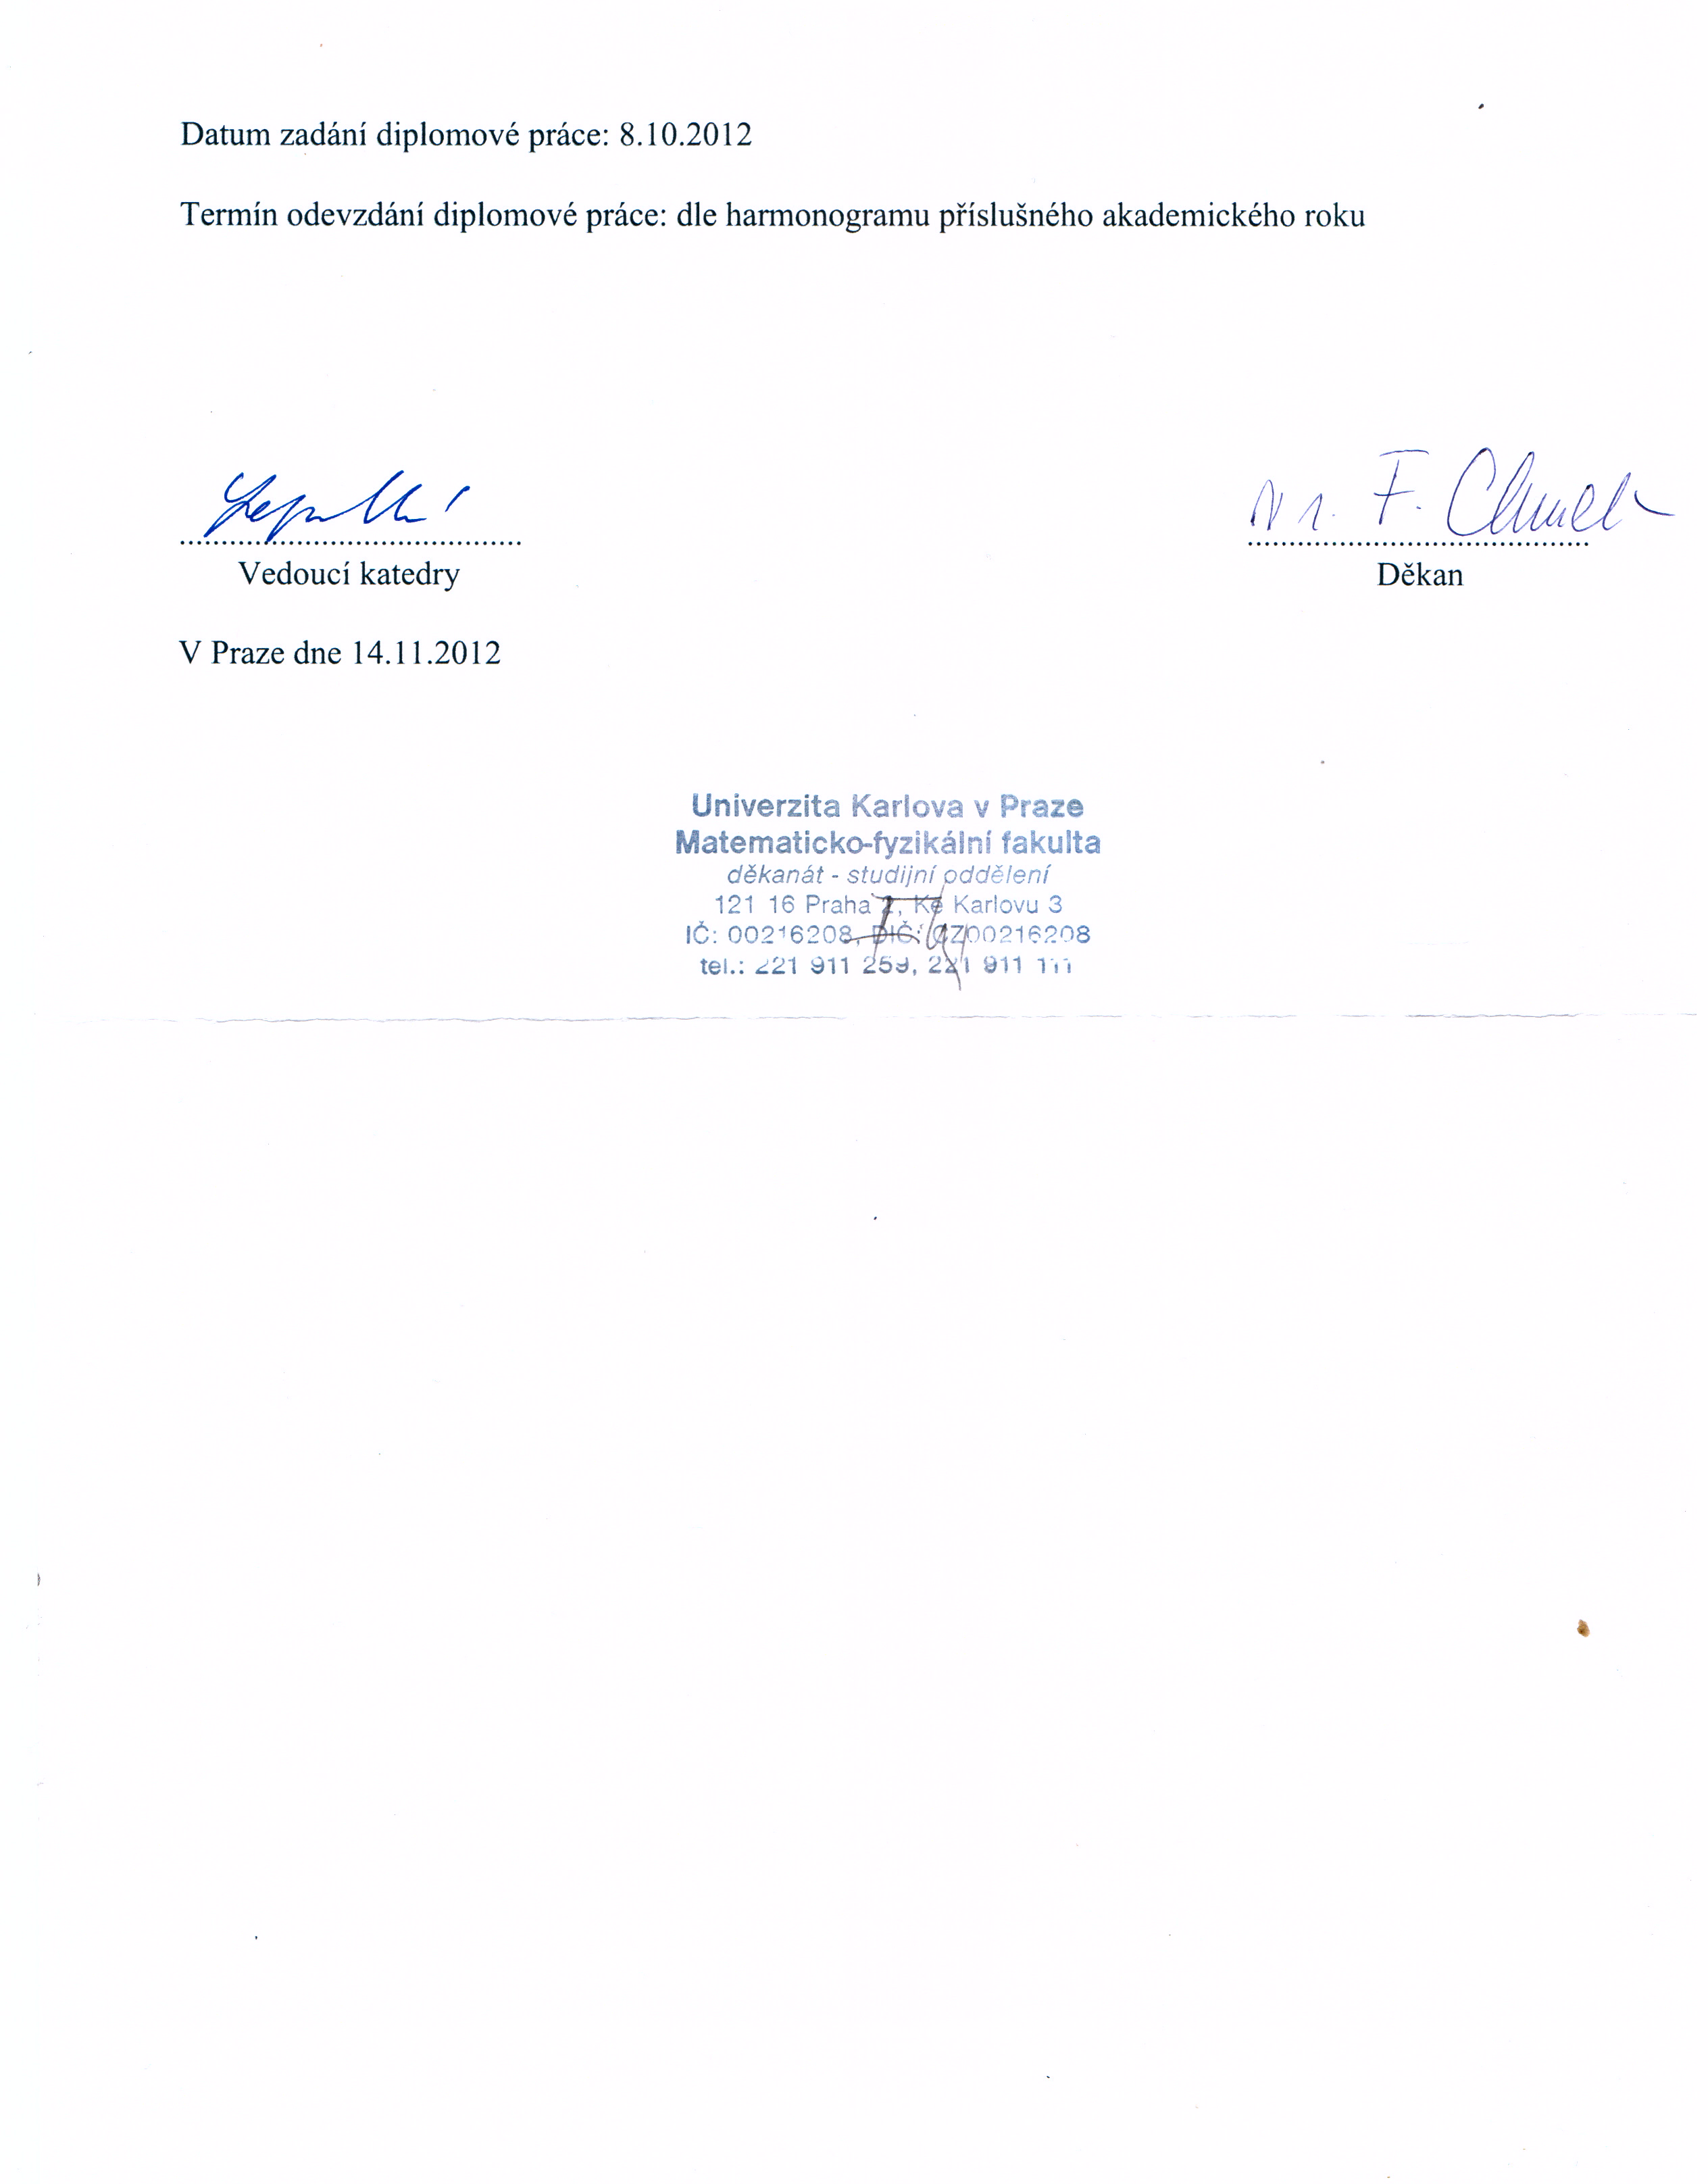
\includegraphics[scale=0.82]{zadani2}}
%\end{figure}  

\newpage

%%% Následuje strana s abstrakty. Doplnte vlastní údaje.
\vbox to 0.5\vsize{
\setlength\parindent{0mm}
\setlength\parskip{5mm}
Název práce: Rozpoznávání řeči pomocí Kaldi\\
Autor: Ondřej Plátek\\
Katedra: Ústav formální a aplikované lingvistiky\\
Vedoucí diplomové práce: Ing. Mgr. Filip Jurčíček, Ph.D.\\
E-mail vedoucího: jurcicek@ufal.mff.cuni.cz\\

\noindent Abstrakt:
Tématem této práce je implementace výkonného rozpoznávače v open-source systému trénování ASR~Kaldi~(\href{http://kaldi.sourceforge.net/}{http://kaldi.sourceforge.net/}) pro dialogové systémy. Kaldi již obsahuje ASR dekodéry, které však nejsou vhodné pro dialogové systémy. 
Hlavními důvody jsou jejich malá optimalizace na rychlost a jejich velké zpoždění v generování výsledku po ukončení promluvy. 
Cílem této práce je proto vyvinutí real-time rozpoznávače pro dialogové systémy optimalizovaného na rychlost a minimalizujícího zpoždění.
 Optimalizace může být realizována například pomocí multi-vláknového dekódování nebo s~využitím grafických karet pro obecné výpočty. 
 Součástí práce je také příprava akustického modelu a testování ve vyvíjeném dialogovém systému ”Vystadial”.


\noindent Klíčová slova: ASR,rozpoznávání mluvené řeči, dekodér

\vspace{10mm}

\noindent
Title: Automatic speech recognition using Kaldi\\
Author: Ondřej Plátek\\
Department: Ústav formální a aplikované lingvistiky \\
Supervisor: Ing. Mgr. Filip Jurčíček, Ph.D.\\
Supervisor's e-mail address: jurcicek@ufal.mff.cuni.cz\\

\noindent Abstract: 
The topic of~this thesis is to implement efficient decoder for speech recognition 
training system ASR~Kaldi~(\href{http://kaldi.sourceforge.net/}{http://kaldi.sourceforge.net/}). 
Kaldi is already deployed with decoders, but they are not convenient for dialog systems. 
The main goal of~this thesis to develop a real-time decoder for a dialog system, 
which minimize latency and optimize speed. Methods used for speeding up the~decoder are not 
limited to multi-threading decoding or usage of~GPU cards for general computations. 
Part of~this work is devoted to training an acoustic model and also testing it in the~"Vystadial" dialog system.

\noindent Keywords: ASR,speech recognition, decoder

\vss}

\newpage

\openright
\pagestyle{plain}
\pagenumbering{arabic}
\setcounter{page}{1}
